\chapter{Introdução}
\textual
A função primaria de um armazém é receber mercadorias de uma fonte, guardar até ser requerido, e enviar para o usuário apropriado quando exigido \cite{tompkins}. É uma parte fundamental da cadeia de suprimentos de qualquer rede de mercadorias.

Nos últimos anos, os armazéns vêm cada vez mais enfrentando maiores demandas por custo e produtividade. Estão se tornando uma parte vital para muitas empresas, porém sua complexidade também está aumentando. Consequentemente, o planejamento e controle dos processos de um armazém, também conhecido como \textit{warehouse management}, tem se tornado uma tarefa desafiadora \cite{faber}.

Nesse contexto, diversas soluções estão sendo buscadas para abaixar os custos, aumentar a produtividade, e melhorar o planejamento dos processos.
Um ponto de melhoria, é a localização de ativos em um armazém. Com dados precisos da localização de todos os ativos em tempo real é possível utilizar algoritmos que visam melhorar a eficiência do armazém.
Os ambientes de armazém, podem ser os mais variados, desde armazéns indoor em ambientes mais controlados, até armazéns outdoor em que espaços são compartilhados entre várias empresas.

Para a realização da localização de produtos em um local indoor e outdoor, diversas tecnologias, técnicas e algoritmos podem ser utilizados, cada um com seus aspectos positivos e negativos, e a escolha de um em detrimento de outro pode levar em conta diversos aspectos. As principais tecnologias utilizadas para a localização são: infravermelho (IR), ultrassom, som audível, sensores magnéticos, sensores óptico, radiofrequência (RF) e luz visível. As tecnologias de RF incluem Bluetooth, banda ultralarga (UWB), wireless sensor network (WSN), rede Local sem fio (WLAN), identificação por radiofrequência (RFID), Near Field Communication (NFC), WiFi, entre outros.
Ja as técnicas de estimativa de localização incluem: Angle of Arrival (AOA), Time of Arrival (TOA), Time Difference of Arrival (TDOA) and Received Signal Strength Indication (RSSI).  \cite{art1,art2}

Essa pesquisa é motivada pela \textit{Samsung SDS Cello Logistics} para a localização de seus ativos em um armazém localizado no Porto de Tubarões no Espirito Santo. Dada a conjuntura do espaço físico de tal porto, somado com os baixos consumos energéticos do Bluetooth, seus baixos custos, e sua alta portabilidade e facilidade de desenvolvimento, tal tecnologia foi escolhida para o desenvolvimento do trabalho, como será demonstrado nas próximas partes.

\section{Necessidade}
\textual
À medida que mais empresas buscam cortar custos e melhorar a produtividade dentro de seus armazéns e centros de distribuição, a etapa de coleta tem se tornado um caso de estudo cada vez mais detalhado. \textit{Order Picking} (Coleta de pedidos) - o processo de coleta de produtos do estoque em resposta ao pedido de um cliente - é a operação mais trabalhosa em armazéns com sistemas manuais e uma operação muito intensiva em armazéns com sistemas automatizados. Por essas razões, os profissionais de armazenamento consideram a coleta de pedidos como a área de prioridade máxima para melhorias de produtividade \cite{art3}.
Nesse contexto de busca de melhorias para a coleta e consequente aumento de produtividade, se encaixam as necessidades do estudo em questão de criar métodos melhores de localização de produtos em um armazém, de forma a otimizar a coleta e estoque de produtos.

No sistema atual, de estoque e coleta do espaço da Samsung, códigos de barra em localidades fixas, são utilizados para a demarcação da localização em que um produto foi estocado. Entretanto, tal método não está se mostrando efetivo em um porto outdoor, com espaços para armazenamento que podem mudar a cada chegada de um novo contêiner e que estão sujeitos a adversidades climáticas. Tal situação exigiu a busca de novas soluções para a localização de produtos a fim de manter padrões elevados de produtividade.


\section{Problema}
\textual
O problema consiste em implementar soluções para a localização de ativos em um espaço físico de um armazém.
O problema de localização outdoor para espaços sem muitos obstáculos, já tem como padrão a tecnologia de GPS, entretanto, quando se trata de espaços outdoor com muitos obstáculos ou espaços indoor, diversas tecnologias são levantadas com aspectos positivos e negativos \cite{art4}, porém a escolha de uma em relação a outra depende do problema em questão

Os principais parâmetros para um sistema ideal de localização, incluem o sistema estar disponivel atualmente em dispositivos de usuários, ser econômico, ser energeticamente eficiente, possuir uma ampla faixa de recepção, alta precisão de localização, baixa latência e alta escalabilidade \cite{art2}.

O problema é que cada tecnologia em conjunto com a aplicação a que se destina pode não apresentar uma ou mais das características ideais desejáveis. Assim, nesse trabalho, será encontrado a solução que melhor se adeque aos parâmetros de um sistema de localização ideal para o armazém específico da Samsung em que o trabalho será feito.

Além disso, o sistema proposto deverá ser facilmente integrável com o \textit{warehouse management system} (WMS) em uso no armazém em questão, de forma a minimizar mudanças na infraestrutura do armazém. Grandes mudanças implicam em custos adicionais, o que é um grande problema em termos comerciais.

\section{Árvore de Objetivos}
Árvore de objetivos: é a representação gráfica do objetivo central do projeto (tronco), dos meios para alcançá-lo (raízes) e dos efeitos positivos que o alcance dos objetivos provoca na população-alvo (galhos e folhas). \cite{Buvinich}

Tal ferramenta é importante para definição de objetivos claros a serem seguidos no projeto e auxiliam no desenvolvimento futuro do projeto.

Na figura \ref{fig:arvore_objetivos} pode-se ver a árvore de objetivos do presente projeto.

\begin{figure}
	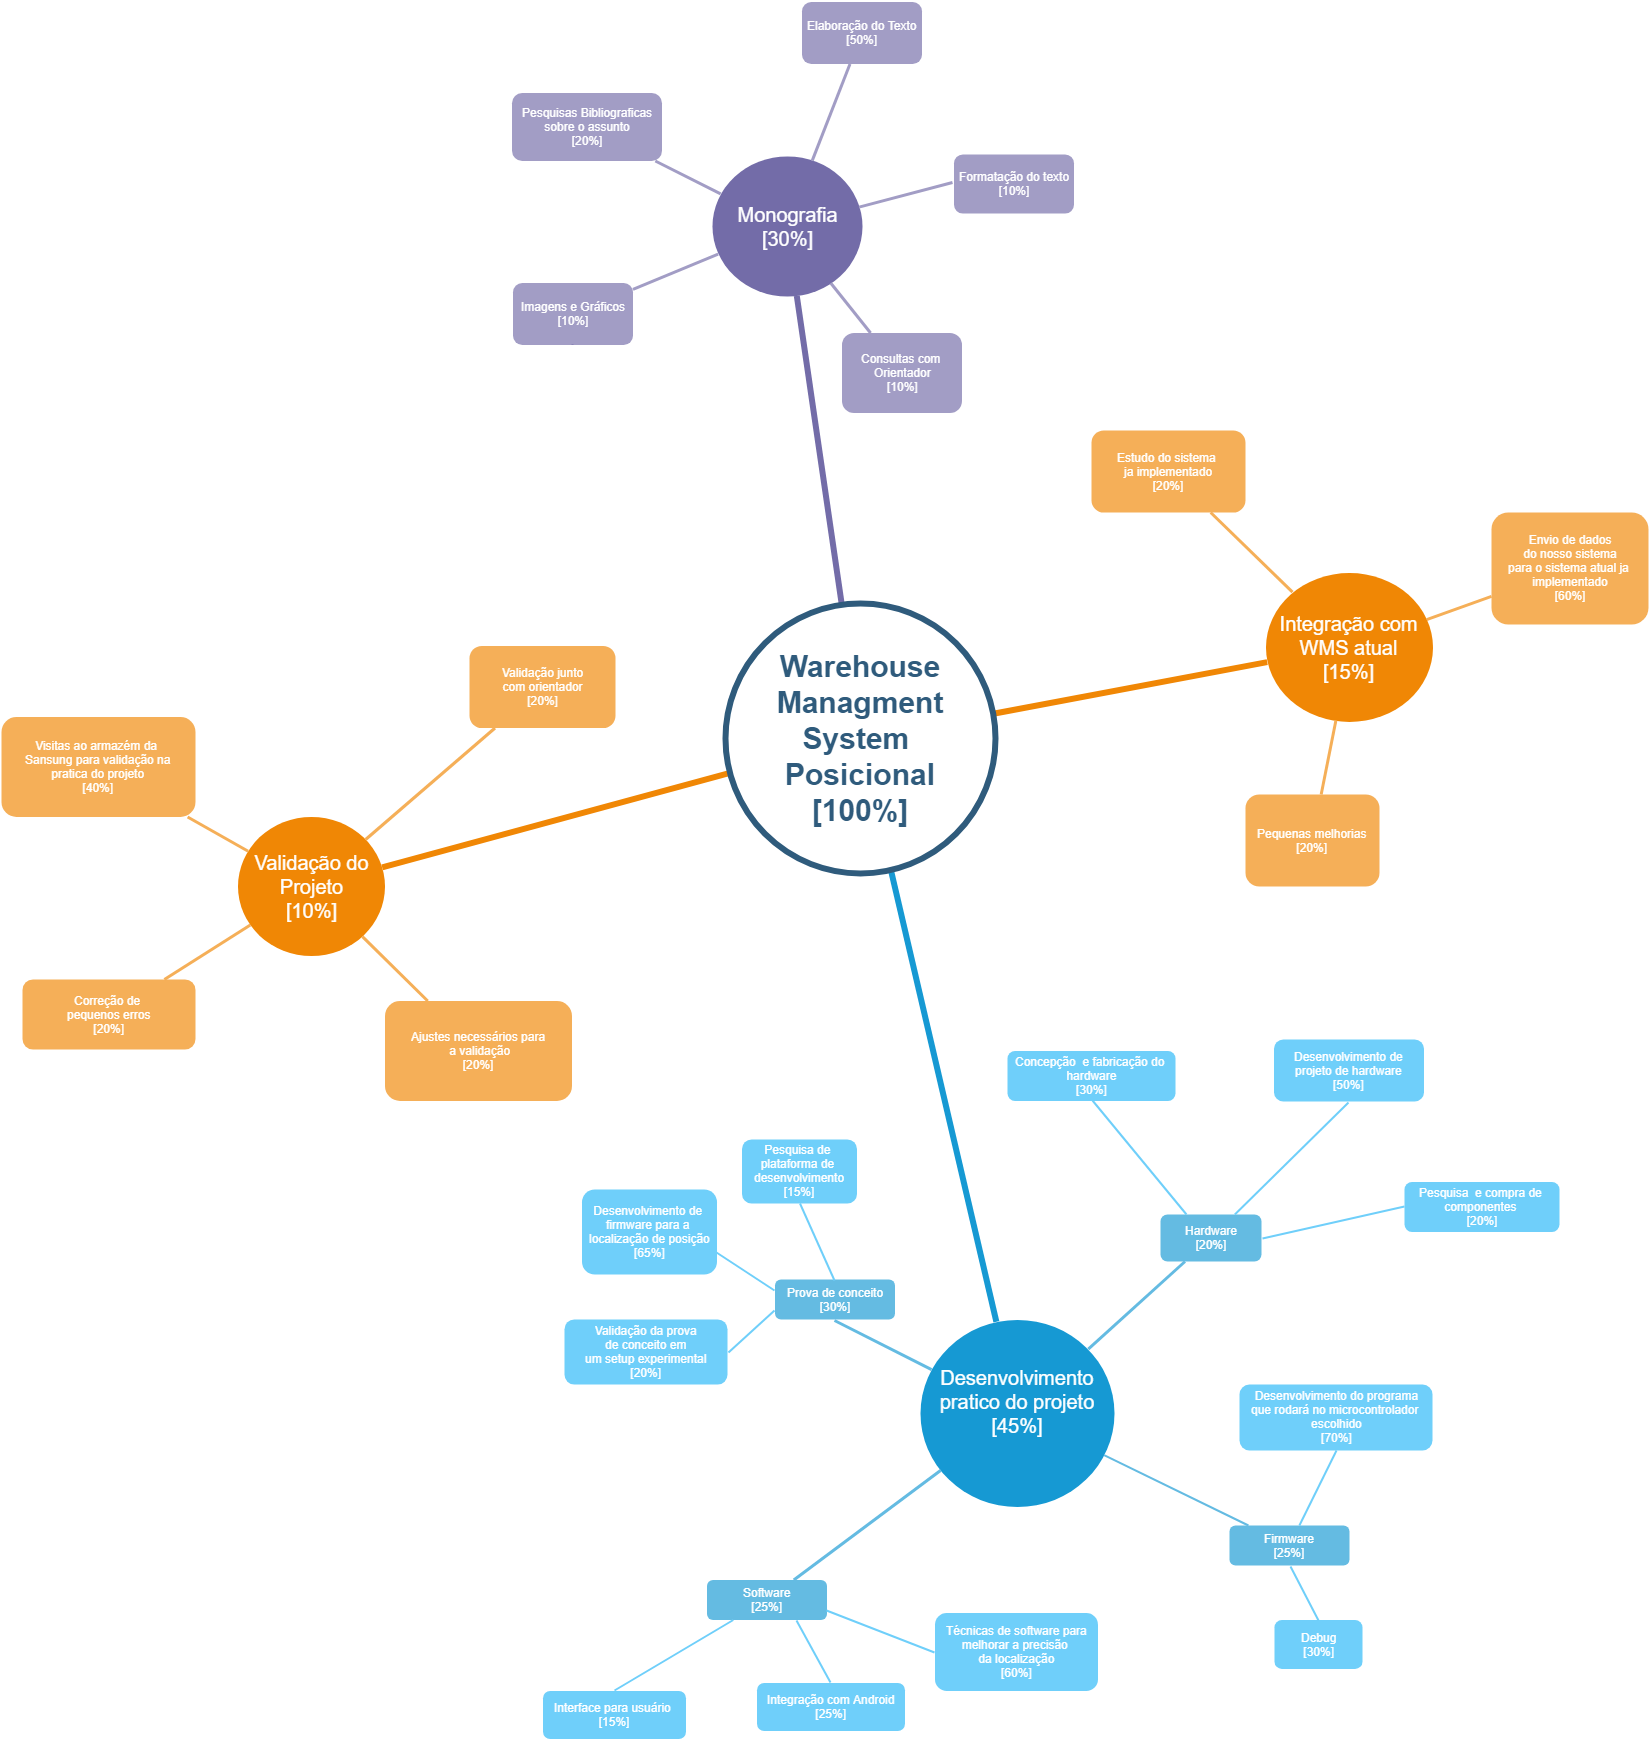
\includegraphics[width=\linewidth]{images/arvore_objetivos.png}
	\caption{Árvore de objetivos do projeto. Em colchetes os tempos de dedicação para cada parte}
	\label{fig:arvore_objetivos}
  \end{figure}
